\documentclass[fontsize=11pt]{article}
\usepackage{amsmath}
\usepackage[utf8]{inputenc}
\usepackage[margin=0.75in]{geometry}
\usepackage{graphicx}
\title{CSC111 Project Proposal: OpenMetroGuide}
\author{Ansh Jain, Nikhil Sreekumar, Sidharth Sachdev}
\date{Tuesday, March 16, 2021}

\begin{document}
\maketitle

\section*{Problem Description and Research Question}

Being a tourist or a non-public-transport user can be difficult especially when trying to figure out the optimum path from your current location to your destination. Looking at the transit maps on the metro lines is not as easy as it seems. Even though places like Toronto and Dubai do not have a complex transit map, places like London and New York City have a web of train stations and tracks. Navigating through these paths can be challenging not only for tourists but also for residents.\newline


\begin{center}
	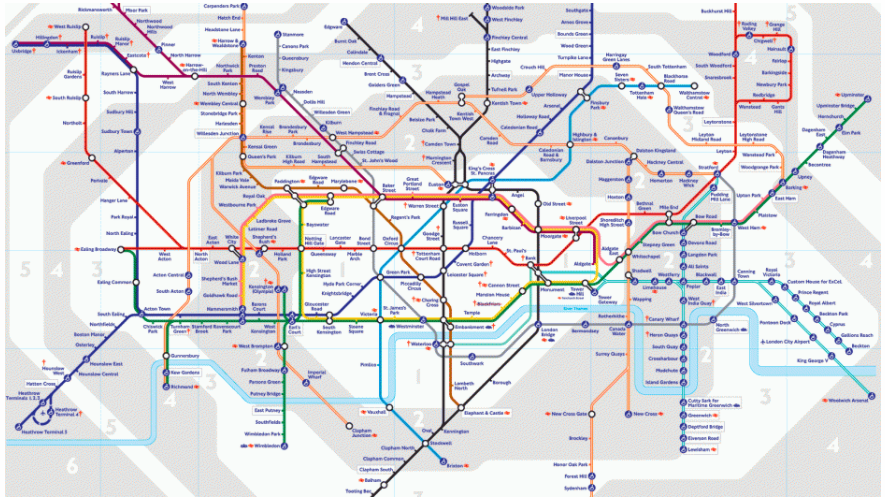
\includegraphics[width = 14cm]{London Transit Map.png}\newline
	London Underground is an example of an extremely complex metro grid.
\end{center}

\textbf{Our project helps its users visualize the best possible path between two stations, based on their preference for a faster or a cheaper route}.\newline 

The objective also includes making the maintaining of the metro map more easier, by providing a set of the most common utilities that would be required. It is clear that this procedure of updating map in real-time (Train delays, stations under maintenance etc.) is a problem that all metros would have to undergo. OpenMetroGuide creates an open standard  based on how the metro stations are maintained and read.\newline



\textbf{
Our project can be a pioneer in using this open standard to make real-time maintenance and use of online metro maps world-wide easier.
}\newline


\section*{Computational Plan}
This application can be accessed by twp types of users. One is the map creator/maintainer and the other is the client using the application for travel information.\\
\\
The map creator will be able to develop the map of that region such as Dubai or Toronto and have the option to edit the map. This will be implemented using the pygame package where the screen will be converted into small grids (similar to the linked list assignment but a lot smaller). The size of these grids will be according to a scale based on the size of the transit map and the creator will be responsible for ensuring this is accurate. The creator will also have the ability to edit the map by having options like adding a new station and adding an edge to connect two stations (with corners to represent/portray a realistic map), all drawn to scale. The map creator will also be responsible for color-coding the lines and also updating the system signifying which paths are not feasible due to factors such as maintenance, traffic, etc. \\
\\
The user interface will consist of an interactive map created with the help of pygame. A complete map of the subway will be displayed on the screen and the user will be able to choose a starting station and a final destination station either by selecting the stations on the interactive map. They will also be able to choose whether they want a time-optimized or a cost-optimized route. Based on these inputs, our application will provide the best route using the A* search algorithm.\\
 \\
We will be using the weighted graph, where the vertices are train stations (with an attribute for direct distance from the destination) and the weighted edges represent the path between adjacent stations with a length attribute. \\
\\
Dijkstra's algorithm is an optimization algorithm to find "the shortest paths between nodes in a graph". This algorithm will be implemented using a priority queue based on the above-mentioned heuristics. The priority queue will be a list of stations ordered based on the cumulated edge lengths combined with either distance from destination or cost. All (unvisited) nodes are initially marked at a distance of infinity from the starting node (which is passed in as the current node). The shortest route will be calculated by prioritizing the distance and edge length whereas the cheapest route will be calculated by giving cost and edge length more importance. Each of the current node's neighbors (except the previously visited ones in the current recursion stack) is given a numeric value based on the weighted edges. Once the destination station is reached, we retrace the stations using recursion till the start/current station which will be the optimum route. \textbf{The A* search algorithm is an extension of this algorithm to help minimize the number of recursive calls made based on an additional "cost" or "overall distance" parameter}.\\
\\
After the best possible path is calculated as per the user's requirements, this application will display the same transit map as described above highlighting the best possible route and blurring the rest of the map. The route will be color-coordinated based on what metro lines have to be taken. The application will also provide the approximate time it takes to reach the destination and a list of the steps to get there with the cost of the ticket.
\section*{References}
\begin{enumerate}
    \item Dijkstra's algorithm. En.wikipedia.org. (2021). https://en.wikipedia.org/wiki/Dijkstra\%27s\_algorithm\#Algorithm.
    \item Dijkstra's Algorithm. Youtube.com. (2017). https://www.youtube.com/watch?v=GazC3A4OQTE.
    \item A* (A Star) Search Algorithm. Youtube.com. (2017). https://www.youtube.com/watch?v=ySN5Wnu88nE\&t=625s.
\end{enumerate}


% NOTE: LaTeX does have a built-in way of generating references automatically,
% but it's a bit tricky to use so we STRONGLY recommend writing your references
% manually, using a standard academic format like APA or MLA.
% (E.g., https://owl.purdue.edu/owl/research_and_citation/apa_style/apa_formatting_and_style_guide/general_format.html)

\end{document}
